\section{Allgemeine Beschreibung}
\subsection{Aufgabenstellung und Umsetzungsansatz}
Die Aufgabestellung des Semesterprojektes ist es eine Hochregallagersimulation unter zuhilfenahme eines Echtzeitbetriebssystems zu erstellen. Diese soll das gesamte System mit einer statisch gewählten Regaldimension sowohl steuern, als auch simulieren.
Das Simulationmodell umfasst ein Regallagersystem mit $5*10$ Regalfächern, einen Ein- und Ausgabeslot und einen Turm zum be- und entladen der Fächer. Dieser Turm ist auf einer Achse montiert, auf welcher er sich in X-Richtung bewegen kann, desweiteren kann der Ausleger am Turm in Y-Richtung herauf und herab bewegen. An dem Ausleger ist widerum ein Schlitten befestigt, welcher in Z-Richtung, zum Hochregal hin, und raus, zu den Ein-/Ausgabe-Slots gefahren werden kann. Die Position dazwischen wird als neutrale Position bezeichnet. Sämtliche Bewegungen des Turms werden von Tastern auf den Schienen ermittelt, um daraus die Position des Turmes bestimmen zu können. Auf der X-Achse und auf der Y-Achse befinden sich jeweils zehn Taster und auf der Z-Achse drei.

Um ein Klötzchen vom Eingabe-Slot, oder aus einem Regalfach aufzunehmen, wird der Schlitten am Ausleger unterhalb des Klötzchens aus der neutralen Position der Z-Achse in den Slot bzw. das Fach gefahren und dann erst angehoben. Umgekehrt wird beim Ablegen eines Klötzchens in den Ausgabe-Slot, oder in ein Regalfach das Paket von oben auf den Slot bzw. das Regalfach abgesenkt, bevor der Ausleger am Schlitten  in die neutrale Position der Z-Achse zurückgefahren wird.
\begin{figure}[H]
	\centering
  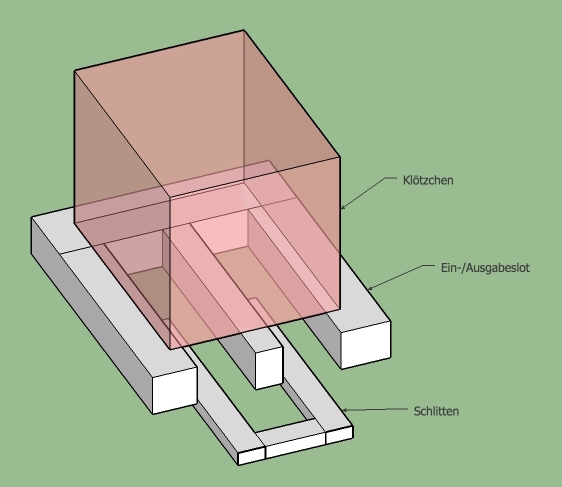
\includegraphics[width=0.45\textwidth]{diagrams/vonunten.jpg}
  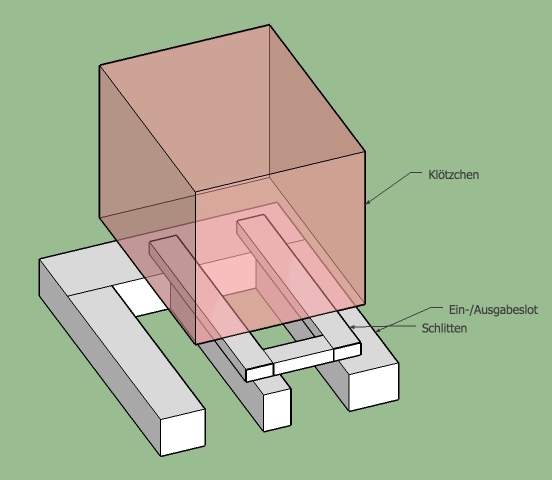
\includegraphics[width=0.45\textwidth]{diagrams/auflegernachoben.jpg}
	\caption{Aufnahme/Ablage an Ein-/Ausgabe-Slot}
	\label{fig2}
\end{figure}

Zur Eingabe steht dem Bediener die Konsole zur Verfügung.
\newline\newline
Folgende Befehle werden zur Verfügung gestellt:
\begin{itemize} 
	\item vsetspace[x][y] $\rightarrow$ Definiert einen Platz als schon belegt
	\item clearspace[x][y] $\rightarrow$ Definiert einen Platz als frei
	\item insert[x][y] $\rightarrow$ Holt ein Klötzchen vom Eingabe-Slot und legt es an gewünschter Position im Hochregallager ab
	\item remove[x][y] $\rightarrow$ Holt ein Klötzchen von der gewünschten Position ab und legt es an den Ausgabe-Slot
\end{itemize}


Sollte ein Befehl nicht möglich sein, da ein Hochregallagerplatz bereits belegt ist bzw. ein Fach aus dem ein Klötzchen geholt werden soll leer ist, wird der Anwender durch eine in der Konsole ausgegebene Fehlermeldung darauf aufmerksam gemacht und der Befehl nicht ausgeführt. Es können vor Abschluss eines Befehls weitere aufgegeben werden, welche sich in einer Warteschlange einreihen. Die Befehle \glqq{} clearspace \grqq{} und \glqq{}vsetspace\grqq{} werden nicht an das Ende dieser gestellt, sondern nach Abschluss des letzten bereits angefangenen Auftrages ausgeführt, da für diese keine Bewegung des Turms nötig ist. Für den Fall, das zu diesem Zeitpunkt eine weitere Operation mit dem selben Regalfach bereits in der Warteschlange ist, welche dieses Fach in einem anderen Belegungszustand benötigt, wird diese dann nicht ausgeführt und der Bediener über das Aussetzen dieses Auftrages mittels Konsolenausgabe informiert.
Sobald kein weiterer Auftrag in der Warteschlange ist wird der Turm an die Position vor dem Eingabe-Slot gefahren und verweilt dort bis ein neuer Auftrag aufgegeben wird.

Die Visualisierung des Hochregallagers erfolgt ebenfalls in der Konsole, in welcher sowohl das Hochregal und dessen Belegung als auch die Position des Turms und dessen Auslegers, durch ASCI-Zeichen stilisiert dargestellt und nach jeder Änderung aktualisiert werden.
Dabei liegt der Ursprung der Koordinaten und somit der Regalplatz (0,0) in der linken unteren Ecke.
Die Darstellung des Ein- und Ausfahren des Auslegers wird unterhalb dargestellt. Dabei stellt die linke Position den zum Ein-/Ausgabe-Slot gefahrenen Arm dar, die rechte Position die in das Regal hereingefahrene. Die aktuelle Position des Turm auf der X- und Y-Achse ist unterhalb bzw. links der Fächer mit einem Pfeil markiert.

\begin{figure}[H]
	\centering
  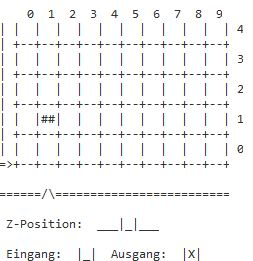
\includegraphics[width=0.5\textwidth]{diagrams/console_output.JPG}
	\caption{Ausgabevisualisierung in Konsole}
	\label{fig3}
\end{figure}

\subsection{Entwicklungsumgebung und Programmierung}
Als Entwicklungs- und Testumgebung wurde Windriver Workbench 3.3 genutz und die Programmiersprache C verwendet.
Es wurden für das Echtzeitbetriebssystem Vxworks Libaries inkludiert und die von Prof. Dr. Jack angebotene Implementierung für die Bus-Datenstruktur (busdata.h) und die User-Befehlseingabe (readcommand.c/.h) verwendet.


